
Negentropy $J(\widehat{s})$ of the reconstructed sources $\widehat{\vec s}$ is defined as:

\begin{equation}
\label{eq:negentropy}
	J(\widehat{s}) \coloneqq H(\widehat{s})_\normal - H(\widehat{s})
\end{equation}

where

\begin{equation}
\label{eq:diffentropyshat}
H(\widehat{s}) := - \int p(\widehat{s}) \log p(\widehat{s}) d\widehat{s}
\end{equation}

\begin{frame} 
\frametitle{Negentropy}
\slidesonly{
$$
H(\hat{s}) := - \int p(\hat{s}) \log p(\hat{s}) d\hat{s} \qquad \qquad \text{(differential entropy)}
$$

\begin{block}{Definition of negentropy}
\begin{equation*}
	J(\widehat{s}) \coloneqq \underbrace{ H(\widehat{s})_\normal}_{
			\substack{ 	\text{entropy of a Gaussian} \\
					\text{distribution with} \\
					\text{same variance}}}
		- \underbrace{ H(\widehat{s}) }_{
			\substack{	\text{entropy of the true} \\
					\text{distribution} \\
					\text{(variance } \sigma^2 \text{)} }}
\end{equation*}
\end{block}
}

\notesonly{
The properties that make negentropy suitable:
}

\begin{itemize}
  \itR theoretically well motivated measure. Considered in some cases the optimzal estimator for nongaussianity.
  \itR non-negative
  \itR scale-invariant: $J(\alpha \widehat{s}) = J(\widehat{s}), \ \ \forall \alpha \ne 0$ (cf. exercise sheet)
  \itR \textbf{Problem:} requires estimation of density $p(\widehat{s})$
\end{itemize}

\question{Should we minimize or maximize negentropy?}

\end{frame}

\subsection{Approximations of negentropy}

\begin{frame}

\notesonly{
Estimating negentropy using the definition in \eqref{eq:negentropy} is computationally costly. It would require estimating the density of the random variable. We therefore resort to simpler approximations for negentropy. Such as the following use of cumulants:
}

\begin{equation}
\label{eq:negentropyapprox}
J(\hat{s}) \approx \frac{1}{12} \langle (\hat{s})^3 \rangle^2 + \frac{1}{48} (\kurt{(\hat{s}))^2} + \text{higher order terms}
\end{equation}

\notesonly{
For symmetric distributions the first term in the approximation in \eqref{eq:negentropyapprox} is effectivley zero, which makes the approximation equivalent to the square of the kurtosis. The approximation would therefore from the same sensitvity to outliers.
}

\slidesonly{
$\rightarrow$ for symmetric distributions optimizing this is equivalent to optimizing $|\kurt{(\hat{s})}|$ sharing its outlier sensitivity \\\vspace{0.4cm}
}
The approximation is modified using 
``nonpolynomial moments'' contrast functions $G$:

\begin{equation}
 J(\hat{s}) \approx \left( \langle G(\hat{s}) \rangle - \langle G(u_{\text{Gauss}}) \rangle \right)^2
\end{equation}

\end{frame}

\clearpage
\begin{frame}{Common contrast functions}
 
 \notesonly{
\textbf{Common contrast functions} 

The contrast function can be chosen depending on the assumed shape of the source densities.

(e.g. speech: highly super-Gaussian)

}
 \begin{figure}
 	\centering
 	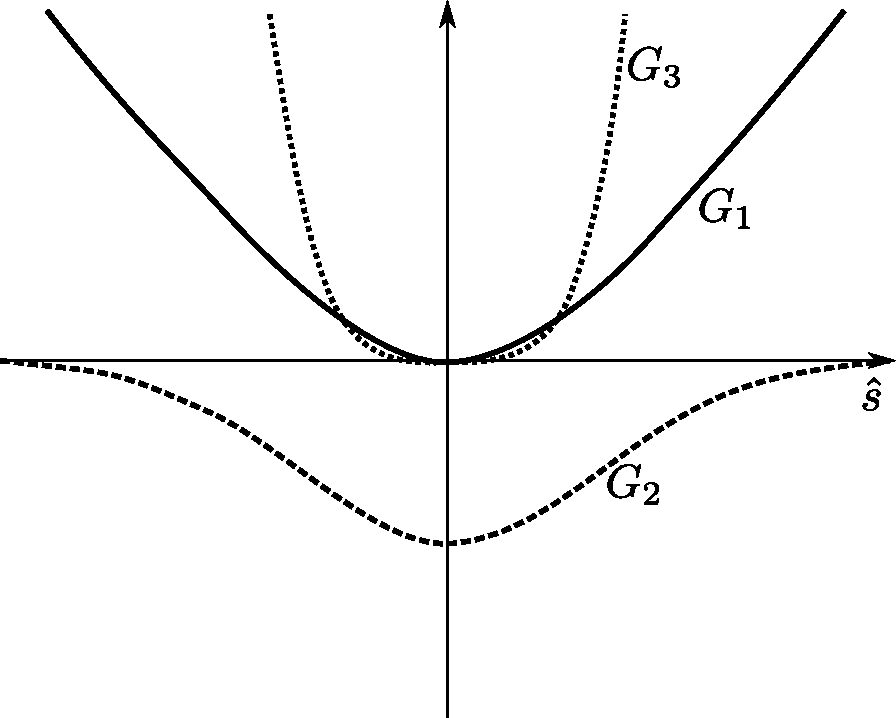
\includegraphics[width=4.5cm]{./img/contrast_functions.pdf}
    \vspace{-0.5cm}
 	\caption*{\hspace{5cm}\textit{\tiny{Source: Hyv\"arinen, 2001}}}
 \end{figure}
 
 \begin{equation*}
 	\smaller
 \begin{array}{lll}
 	G_1(\hat{s}) = \frac{1}{a} \log \cosh (a \cdot \hat{s}) 
 	\;\;& \;\;G_2(\hat{s}) = -\exp \Big( -\frac{(\hat{s})^2}{2} \Big)
 	& \;\;G_3(\hat{s}) = \frac{1}{4} (\hat{s})^4
	\end{array}
 \end{equation*}
 Any even, non-constant and non-quadratic (contrast) function $G$ can be used for ICA
 
 \question{When to choose which contrast function?}
 
 \end{frame}

\begin{frame}
\slidesonly{
\frametitle{Common contrast functions:}
}
\slidesonly{
	\smaller
	\begin{tabular}{ccc}
		$G_1(\hat{s}) = \frac{1}{a} \log \cosh (a \cdot \hat{s})$ & $G'_1(\hat{s}) = \tanh{(a\hat{s})}$ & $G''_1(\hat{s}) = a (1 - \tanh^2{(a\hat{s})})$\\[7pt]
		\multicolumn{3}{c}{general purpose} \\[25pt]
		$G_2(\hat{s}) = -\exp \Big( -\frac{(\hat{s})^2}{2} \Big)$ & $G'_2(\hat{s}) = \hat{s} \exp{(-\frac{(\hat{s})^2}{2})}$ & $G''_2(\hat{s}) = (1-(\hat{s})^2) \exp{(-\frac{(\hat{s})^2}{2})}$ \\[7pt]
		\multicolumn{3}{c}{good for ``super''-Gaussian sources with many ``outliers''} \\[25pt]
		$G_3(\hat{s}) = \frac{1}{4} (\hat{s})^4 $ & $G'_3(\hat{s}) = (\hat{s})^3$ & $G''_3(\hat{s}) = 3(\hat{s})^2$  \\[7pt]
		\multicolumn{3}{c}{kurtosis: good for ``sub''-Gaussian sources with few ``outliers''}
	\end{tabular}
}
\notesonly{
\begin{itemize}
    \item general purpose:
    \begin{itemize}
        \item $G_1(\hat{s}) = \frac{1}{a} \log \cosh (a \cdot \hat{s})$
        \item $G'_1(\hat{s}) = \tanh{(a\hat{s})}$
        \item $G''_1(\hat{s}) = a (1 - \tanh^2{(a\hat{s})})$
    \end{itemize}
    \item for ``super''-Gaussian sources with many ``outliers'':
    \begin{itemize}
        \item $G_2(\hat{s}) = -\exp \Big( -\frac{(\hat{s})^2}{2} \Big)$
        \item $G'_2(\hat{s}) = \hat{s} \exp{(-\frac{(\hat{s})^2}{2})}$
        \item $G''_2(\hat{s}) = (1-(\hat{s})^2) \exp{(-\frac{(\hat{s})^2}{2})}$
    \end{itemize}
    \item kurtosis: good for ``sub''-Gaussian sources with few ``outliers'':
    \begin{itemize}
        \item $G_3(\hat{s}) = \frac{1}{4} (\hat{s})^4 $
        \item $G'_3(\hat{s}) = (\hat{s})^3$
        \item $G''_3(\hat{s}) = 3(\hat{s})^2$
    \end{itemize}
\end{itemize}
}
\end{frame}

\begin{frame}
cf. lecture slides for optmization of negentropy using contrast functions.
\end{frame}

\begin{frame}
\question{How do we evaluate ICA?}\\

-cf. https://research.ics.aalto.fi/ica/icasso/
\end{frame}

